% ======================================================================
% 8. přednáška (21. 11. 2022) – kvarkový model (pokračování), leptony,
% interakce a Feynmanovy diagramy, narušení P a CP, neutrální kaony
% ======================================================================
\tikzset{
  jcosm foton/.style={decorate,decoration={snake,amplitude=1.6pt,segment length=6pt}},
  jcosm gluon/.style={decorate,decoration={coil,aspect=0.7,amplitude=2.4pt,segment length=4pt}},
  jcosm bod/.style={circle,fill,inner sep=1.3pt}
}

\section{Kvarkový model -- pokračování: šest kvarků, leptony a interakce}

\strana{P08-1}
\subsection{Objev \texorpdfstring{$J/\psi$}{J/psi}}

Na minulé přednášce jsme sestavili kvarkový model ze tří lehkých kvarků $u$, $d$, $s$, který vysvětlil oktety a dekuplet hadronů. Celkový obraz se ale v listopadu 1974 změnil -- dvě nezávislé skupiny téměř současně objevily novou, velmi úzkou rezonanci, kterou dnes nazýváme \kw{$J/\psi$} (dvojí jméno je pozůstatkem toho, že ji každá skupina pojmenovala jinak; v historii se tomu říká \uv{listopadová revoluce}). Její parametry jsou
\begin{equation}
  m(J/\psi) \approx 3{,}1\,\mathrm{GeV}, \qquad \Gamma(J/\psi) \doteq 93\,\mathrm{keV}.
\end{equation}
Zde $m$ je klidová hmotnost a $\Gamma$ je \kw{rozpadová šířka}, tj.\ šířka rezonančního píku v~energii, která souvisí se střední dobou života vztahem $\tau = \hbar/\Gamma$. Pro $\Gamma = 93\,\mathrm{keV}$ vychází $\tau \approx 6{,}6\cdot 10^{-16}\,\mathrm{eV\,s}/93\cdot10^{3}\,\mathrm{eV}\approx 7\cdot 10^{-21}\,\mathrm{s}$. To je na hadron s hmotností přes $3\,\mathrm{GeV}$, který se rozpadá silnou interakcí, \pozor{neobyčejně dlouho} -- typické silně se rozpadající rezonance (např.\ $\rho$, $\Delta$) mají šířky stovek MeV, tedy o tři až čtyři řády větší. Právě tato úzkost byla hlavní záhadou a zároveň klíčem k~interpretaci.

Rezonanci bylo vidět ve dvou zcela odlišných typech experimentů:
\begin{itemize}
  \item \textbf{SLAC} (B.~Richter) -- srážky $e^+ + e^- \to X$: měří se účinný průřez produkce hadronů v~závislosti na celkové energii v~těžišti $\sqrt{s}$. Pokud se $\sqrt{s}$ trefí do hmotnosti nějaké částice, která se může vytvořit z~$e^+e^-$ (přes virtuální foton), účinný průřez prudce vyskočí -- vznikne rezonanční pík.
  \item \textbf{BNL} (S.~Ting) -- srážky protonů s~pevným terčíkem z~berylia $p + \mathrm{Be} \to e^+ e^- + X$: zde se v~každé události změří páry $e^+e^-$ a z~jejich hybností se dopočte \kw{invariantní hmotnost} páru $m_{ee}$. Pokud pár pochází z~rozpadu částice, $m_{ee}$ je rovna její hmotnosti, takže v~histogramu $m_{ee}$ se objeví pík nad hladkým pozadím.
\end{itemize}

\begin{center}
\begin{tikzpicture}[>=Stealth]
  % e+e- -> X
  \draw[->] (0,0) -- (4.2,0) node[below left]{$\sqrt{s}$};
  \draw[->] (0,0) -- (0,2.8) node[left]{$\sigma$};
  \draw[thick] (0.25,2.5) .. controls (0.9,1.3) and (1.8,0.75) .. (2.55,0.72)
     .. controls (2.75,0.75) and (2.85,1.4) .. (2.9,1.75)
     .. controls (2.95,1.2) and (3.05,0.7) .. (4.0,0.4);
  \draw[dashed] (2.9,1.75) -- (2.9,0) node[below]{$m$};
  \node at (2,3.1) {$e^+ + e^- \to X$};
  % p+Be
  \begin{scope}[xshift=6cm]
  \draw[->] (0,0) -- (4.2,0) node[below left]{$m_{ee}$};
  \draw[->] (0,0) -- (0,2.8) node[left]{$\dd N/\dd m_{ee}$};
  \draw[thick] (0.3,2.0) .. controls (0.8,1.0) and (1.3,0.65) .. (1.65,0.7)
     .. controls (1.85,0.8) and (1.95,1.6) .. (2.0,2.3)
     .. controls (2.05,1.2) and (2.15,0.75) .. (2.3,0.65)
     .. controls (2.8,0.45) and (3.4,0.45) .. (4.0,0.45);
  \draw[dashed] (2.0,2.3) -- (2.0,0) node[below]{$m$};
  \node at (2,3.1) {$p + \mathrm{Be} \to e^+e^- + X$};
  \end{scope}
\end{tikzpicture}
\end{center}

Oba experimenty dávají pík na stejné hmotnosti $m\approx3{,}1\,\mathrm{GeV}$, takže jde o~tutéž částici. Interpretace: $J/\psi$ je vázaný stav nového, čtvrtého kvarku $c$ (\kw{půvabný kvark}, \emph{charm}) a jeho antikvarku,
\begin{equation}
  \vzorec{J/\psi = (c\bar c)}, \qquad m(J/\psi) < 2m(D).
\end{equation}
Nerovnost vysvětluje malou šířku. Nejsnazší silný rozpad by byl takový, při němž se kvarky $c$ a $\bar c$ \uv{rozejdou} každý do jiného mezonu -- do páru mezonů $D$ ($D = c\bar u$, $c\bar d$ apod., $m(D)\approx 1{,}87\,\mathrm{GeV}$). Jenže $2m(D)\approx 3{,}73\,\mathrm{GeV} > 3{,}1\,\mathrm{GeV}$, takže tento kanál je energeticky zakázán. $J/\psi$ se proto musí rozpadnout tak, že $c$ a $\bar c$ spolu anihilují (na gluony nebo foton), a tento proces je silně potlačen (tzv.\ \kw{OZI pravidlo}). Odtud dlouhá doba života a úzký pík.

\begin{vysvetleni}[Proč je $J/\psi$ vidět jako úzký pík i v $e^+e^-$]
  $J/\psi$ má spin a paritu $J^{PC}=1^{--}$, stejně jako foton. Může tedy vzniknout přímo z~anihilace $e^+e^-$ přes virtuální foton, a naopak se s~nezanedbatelnou pravděpodobností rozpadá zpět na leptonový pár $e^+e^-$ nebo $\mu^+\mu^-$ (to využil Ting). Na Davídkových slajdech (kapitola o~kvarkovém modelu, měření $R=\sigma(e^+e^-\to\text{hadrony})/\sigma(e^+e^-\to\mu^+\mu^-)$) je vidět, že nad prahem produkce kvarku $c$ poměr $R$ vzroste -- přibyl další kvark, který lze v~anihilaci vytvořit.
\end{vysvetleni}

\strana{P08-2}
\subsection{Šest kvarků}

Postupně (1977 kvark $b$ v~rezonanci $\Upsilon=b\bar b$, 1995 kvark $t$ ve Fermilabu) se ukázalo, že kvarků je \textbf{nakonec šest}. Uspořádáváme je do tří \kw{generací} (rodin), každá generace obsahuje jeden kvark s~nábojem $+\tfrac23$ a jeden s~nábojem $-\tfrac13$ (v~jednotkách elementárního náboje $e$):
\begin{center}
\begin{tikzpicture}
  \node at (0,0.5) {$u$}; \node at (1.2,0.5) {$c$}; \node at (2.4,0.5) {$t$};
  \node at (0,-0.5) {$d$}; \node at (1.2,-0.5) {$s$}; \node at (2.4,-0.5) {$b$};
  \draw (-0.6,0) -- (3.0,0);
  \foreach \x in {0,1.2,2.4} \draw[ForestGreen] (\x,0) ellipse (0.42 and 1.0);
  \node[left] at (-0.7,0) {$\left(\vphantom{\rule{0pt}{1.0cm}}\right.$};
  \node[right] at (3.0,0) {$\left.\vphantom{\rule{0pt}{1.0cm}}\right)$};
  \node[right] at (3.6,0.5) {$q = +\tfrac{2}{3}$};
  \node[right] at (3.6,-0.5) {$q = -\tfrac{1}{3}$};
  \node[right] at (6.0,0.5) {$m(t) \approx 175\,\mathrm{GeV}$};
\end{tikzpicture}
\end{center}
\pozn{v originále lze číst „145“ i „175 GeV“; dnešní hodnota je $m_t\approx173\,\mathrm{GeV}$, proto čteno 175} Zelené ovály v~poznámkách vyznačují generace: $(u,d)$, $(c,s)$, $(t,b)$. Hmotnosti rostou od generace ke generaci, a to dramaticky: $u$, $d$ mají jednotky MeV, $s$ asi $100\,\mathrm{MeV}$, $c\approx1{,}3\,\mathrm{GeV}$, $b\approx4{,}2\,\mathrm{GeV}$ a \kw{top kvark} má hmotnost $m(t)\approx 175\,\mathrm{GeV}$ -- je tak těžký jako atom zlata. Důsledkem je, že $t$ se rozpadne (slabou interakcí, $t\to bW^+$) dřív, než stihne vytvořit hadron; je to jediný kvark, který nikdy nepozorujeme vázaný v~hadronech.

\subsection{Hadronizace}

Kvarky nikdy nevidíme volné (\kw{uvěznění}, \emph{confinement}). Co se tedy stane, když kvarkový pár vytvoříme, například v~anihilaci $e^+e^- \to \gamma^* \to q\bar q$? Kvark a antikvark se od sebe rozlétají s~velkou energií. Mezi nimi se natahuje barevné pole -- \uv{struna} gluonového pole, jejíž energie roste přibližně lineárně se vzdáleností. Jakmile je energie uložená ve struně dostatečná, je energeticky výhodnější, aby struna \uv{praskla} a z~vakua vznikl nový pár $q'\bar q'$. Proces se opakuje (vzniká $q''\bar q''$, \dots), až má každý úsek tak malou energii, že se kvarky a antikvarky sdruží do bezbarvých hadronů. Tomuto procesu se říká \kw{hadronizace}.
\begin{center}
\begin{tikzpicture}[>=Stealth]
  \coordinate (em) at (-2.2,-1.0); \coordinate (ep) at (-2.2,1.0);
  \coordinate (v1) at (-1.2,0); \coordinate (v2) at (0.4,0);
  \coordinate (q) at (3.2,2.4); \coordinate (qb) at (3.2,-2.4);
  \draw[thick] (ep) -- (v1) node[pos=0,left]{$e^+$};
  \draw[thick] (em) -- (v1) node[pos=0,left]{$e^-$};
  \draw[thick,jcosm foton] (v1) -- (v2) node[midway,above=2pt]{$\gamma$};
  \draw[thick] (v2) -- (q) node[pos=0.45,above left]{$q$};
  \draw[thick] (v2) -- (qb) node[pos=0.45,below left]{$\bar q$};
  % struna
  \draw[gray] (2.45,1.75) .. controls (2.3,0.5) and (2.6,-0.5) .. (2.45,-1.75);
  \draw[gray] (2.7,1.95) .. controls (2.55,0.5) and (2.85,-0.5) .. (2.7,-1.95);
  % zlomy struny
  \draw[red,thick] (2.25,0.85) -- (2.95,0.85); \draw[red,thick] (2.25,0.75) -- (2.95,0.75);
  \draw[red,thick] (2.25,-0.65) -- (2.95,-0.65); \draw[red,thick] (2.25,-0.75) -- (2.95,-0.75);
  \node[red,right] at (2.95,0.95) {$\bar q'$}; \node[red,right] at (2.95,0.55) {$q'$};
  \node[red,right] at (2.95,-0.55) {$\bar q''$}; \node[red,right] at (2.95,-0.95) {$q''$};
  % hadrony
  \draw[ForestGreen] (2.6,1.65) ellipse (0.45 and 0.9);
  \draw[ForestGreen] (2.6,0.05) ellipse (0.4 and 0.65);
  \draw[ForestGreen] (2.6,-1.55) ellipse (0.45 and 0.85);
\end{tikzpicture}
\end{center}
V~obrázku: $e^+e^-$ anihilují na virtuální foton, ten vytvoří pár $q\bar q$; zvlněné čáry mezi rozlétajícími se kvarky představují barevnou strunu, červené dvojčárky místa, kde se struna přetrhne a vznikne pár $\bar q' q'$, resp.\ $\bar q'' q''$. Zelené ovály ohraničují výsledné bezbarvé hadrony (zde tři mezony: $q\bar q'$, $q'\bar q''$, $q''\bar q$). V~detektoru pak místo kvarků pozorujeme úzké svazky hadronů letící zhruba ve směru původních kvarků -- \kw{jety}.

\subsection{Leptony}

Druhou skupinou základních fermionů (spin $\tfrac12$) jsou \kw{leptony} -- částice, které necítí silnou interakci. Také je jich šest a také tvoří tři generace:
\begin{center}
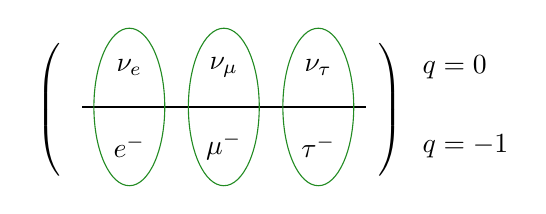
\begin{tikzpicture}
  \node at (0,0.5) {$\nu_e$}; \node at (1.2,0.5) {$\nu_\mu$}; \node at (2.4,0.5) {$\nu_\tau$};
  \node at (0,-0.5) {$e^-$}; \node at (1.2,-0.5) {$\mu^-$}; \node at (2.4,-0.5) {$\tau^-$};
  \draw (-0.6,0) -- (3.0,0);
  \foreach \x in {0,1.2,2.4} \draw[ForestGreen] (\x,0) ellipse (0.45 and 1.0);
  \node[left] at (-0.7,0) {$\left(\vphantom{\rule{0pt}{1.0cm}}\right.$};
  \node[right] at (3.0,0) {$\left.\vphantom{\rule{0pt}{1.0cm}}\right)$};
  \node[right] at (3.6,0.5) {$q = 0$};
  \node[right] at (3.6,-0.5) {$q = -1$};
\end{tikzpicture}
\end{center}
Nabité leptony $e^-$, $\mu^-$, $\tau^-$ mají náboj $-1$ a hmotnosti $0{,}511\,\mathrm{MeV}$, $105{,}7\,\mathrm{MeV}$ a $1777\,\mathrm{MeV}$; neutrina jsou neutrální a velmi lehká. Ke každému leptonu existuje antilepton ($e^+$, $\bar\nu_e$, \dots).

Pozorování ukazují, že se zachovává počet leptonů -- a to dokonce pro každou generaci zvlášť. Zavádíme proto \kw{leptonová čísla} $L_e$, $L_\mu$, $L_\tau$. Pro elektronovou rodinu
\begin{equation}
  L_e(e^-) = 1, \quad L_e(\nu_e) = 1, \qquad L_e(e^+) = -1, \quad L_e(\bar\nu_e) = -1,
\end{equation}
ostatní částice mají $L_e=0$; analogicky pro $L_\mu$, $L_\tau$. Proto se v~rozpadu neutronu $n\to p+e^-+\bar\nu_e$ vytváří právě \emph{anti}neutrino: $L_e$ je před rozpadem $0$ a po rozpadu $1+(-1)=0$. (Zachování jednotlivých $L_e$, $L_\mu$, $L_\tau$ je ve skutečnosti narušeno oscilacemi neutrin, celkové $L$ se ale zachovává.)

\strana{P08-3}
\subsection{Interakce}

Známe tedy \uv{stavební kameny} hmoty. Jak spolu interagují? V~kvantové teorii pole se interakce popisuje \kw{pomocí výměny bosonů} (nositelů interakce, se spinem 1) a názorně se zakresluje \kw{Feynmanovými diagramy}. Čas v~našich diagramech poběží zleva doprava; plné čáry jsou fermiony (kvarky, leptony), vlnovky intermediální bosony, tečky jsou \kw{vrcholy} (vertexy), v~nichž boson interaguje s~fermiony. Každému vrcholu odpovídá ve výpočtu amplitudy jeden faktor vazbové konstanty (pro elektromagnetickou interakci $\sqrt{\alpha}$, $\alpha\approx1/137$), takže diagramy s~méně vrcholy obvykle dominují.

\begin{vysvetleni}[Proč výměna částice znamená sílu]
  Virtuální boson s~hmotností $M$ si podle relace neurčitosti může \uv{vypůjčit} energii $Mc^2$ na dobu $\Delta t\sim\hbar/(Mc^2)$, a uletí tak nejvýše vzdálenost $R\sim c\Delta t = \hbar/(Mc)$. Odtud dosah interakce: nehmotný foton $\Rightarrow$ nekonečný dosah ($1/r$ potenciál), pion $m_\pi\approx140\,\mathrm{MeV}$ $\Rightarrow$ $R\approx1{,}4\,\mathrm{fm}$ (jaderné síly), $W$, $Z$ s~$m\approx80$--$90\,\mathrm{GeV}$ $\Rightarrow$ $R\approx 2\cdot10^{-3}\,\mathrm{fm}$ (slabá interakce je \uv{bodová}). Tuto úvahu (Yukawa) jsme potkali už u jaderných sil.
\end{vysvetleni}

\subsection{Elektromagnetická interakce}

Nositelem elektromagnetické interakce je \kw{foton} $\gamma$, nehmotný boson se spinem $S(\gamma)=1$. Foton se váže na elektrický náboj -- tedy na všechny nabité fermiony -- a sám náboj nenese. Typickým procesem je anihilace $e^+e^-\to\mu^+\mu^-$:
\begin{center}
\begin{tikzpicture}[>=Stealth]
  \coordinate (a) at (0,0); \coordinate (b) at (2,0);
  \node[jcosm bod] at (a) {}; \node[jcosm bod] at (b) {};
  \draw[thick] (-1.2,1) -- (a) node[pos=0,left]{$e^-$};
  \draw[thick,->] (-1.2,1) -- (-0.6,0.5);
  \draw[thick] (-1.2,-1) -- (a) node[pos=0,left]{$e^+$};
  \draw[thick,->] (a) -- (-0.6,-0.5);
  \draw[thick,jcosm foton] (a) -- (b) node[midway,below=3pt]{$\gamma$};
  \draw[thick] (b) -- (3.2,1) node[right]{$\mu^-$};
  \draw[thick,->] (b) -- (2.6,0.5);
  \draw[thick] (b) -- (3.2,-1) node[right]{$\mu^+$};
  \draw[thick,->] (3.2,-1) -- (2.6,-0.5);
  % zakázaný vrchol 3 fotonů
  \begin{scope}[xshift=7cm]
    \coordinate (c) at (0,0);
    \draw[thick,jcosm foton] (-1.3,0) -- (c) node[pos=0,left]{$\gamma$};
    \draw[thick,jcosm foton] (c) -- (0.8,0.9) node[right]{$\gamma$};
    \draw[thick,jcosm foton] (c) -- (0.1,-1.1) node[below]{$\gamma$};
    \node[jcosm bod] at (c) {};
    \draw[red,very thick] (-1.0,-1.0) -- (1.0,1.0);
    \draw[red,very thick] (-0.9,1.0) -- (1.0,-0.9);
  \end{scope}
\end{tikzpicture}
\end{center}
Šipky u fermionů ukazují tok fermionového (leptonového) čísla; antičástice má šipku proti směru času. V~levém vrcholu $e^-$ a $e^+$ zaniknou a vznikne (virtuální) foton, v~pravém foton vytvoří pár $\mu^-\mu^+$. Každý vrchol zachovává náboj i leptonová čísla.

Vpravo přeškrtnutý diagram říká důležitou věc: \pozor{neexistuje vrchol, v~němž by se setkaly tři fotony} (a ani čtyři). Foton nemá náboj, a tak sám se sebou přímo neinteraguje -- elektromagnetická teorie je \emph{lineární} (proto platí princip superpozice v~klasické elektrodynamice).

\strana{P08-4}
Fotony spolu přesto mohou interagovat nepřímo, přes smyčku virtuálních nabitých částic. Rozptyl světla na světle $\gamma\gamma\to\gamma\gamma$ probíhá nejníže diagramem se čtyřmi vrcholy, v~němž fotony interagují s~uzavřenou elektronovou smyčkou:
\begin{center}
\begin{tikzpicture}[>=Stealth]
  \coordinate (A) at (0,1); \coordinate (B) at (1.5,1);
  \coordinate (C) at (1.5,0); \coordinate (D) at (0,0);
  \draw[thick,jcosm foton] (-1.6,1) -- (A) node[pos=0,left]{$\gamma$};
  \draw[thick,jcosm foton] (B) -- (3.1,1) node[right]{$\gamma$};
  \draw[thick,jcosm foton] (-1.6,0) -- (D) node[pos=0,left]{$\gamma$};
  \draw[thick,jcosm foton] (C) -- (3.1,0) node[right]{$\gamma$};
  \draw[thick] (A) -- (B) -- (C) -- (D) -- cycle;
  \draw[thick,->] (A) -- (0.85,1) node[above]{$e^-$};
  \draw[thick,->] (B) -- (1.5,0.45);
  \draw[thick,->] (C) -- (0.65,0);
  \draw[thick,->] (D) -- (0,0.55) node[left]{$e^-$};
  \foreach \p in {A,B,C,D} \node[jcosm bod] at (\p) {};
\end{tikzpicture}
\end{center}
Protože obsahuje čtyři vrcholy, je amplituda úměrná $\alpha^2$ a účinný průřez $\alpha^4$ -- rozptyl světla na světle je proto extrémně slabý, ale je pozorován (např.\ v~ultraperiferních srážkách těžkých iontů na LHC).

\subsection{Silná interakce}

\paragraph{Jaderné síly jako výměna pionu.}
Na úrovni nukleonů jsme silnou interakci popisovali (Yukawovým) mechanismem výměny pionů. Například proton a neutron si mohou vyměnit nabitý pion $\pi^+$: proton jej vyzáří a změní se na neutron, neutron jej pohltí a stane se protonem, $p+n\to n+p$:
\begin{center}
\begin{tikzpicture}[>=Stealth]
  \draw[thick] (0,1.2) -- (4,1.2); \draw[thick] (0,0) -- (4,0);
  \node[left] at (0,1.2) {$p$}; \node[right] at (4,1.2) {$n$};
  \node[left] at (0,0) {$n$}; \node[right] at (4,0) {$p$};
  \draw[thick,dashed] (2,1.2) -- (2,0) node[midway,right]{$\pi^+$};
  \node[jcosm bod] at (2,1.2) {}; \node[jcosm bod] at (2,0) {};
\end{tikzpicture}
\end{center}
Pion je však sám složený (ze dvojice $u\bar d$), takže tento obraz je jen efektivní. Fundamentální teorií silné interakce je \kw{kvantová chromodynamika} (QCD): nositeli jsou \kw{gluony} $g$ (nehmotné, spin 1), které se vážou na \kw{barevný náboj} kvarků. Na rozdíl od fotonu nesou gluony samy barvu (kombinaci barvy a antibarvy, celkem 8 druhů), a proto
\begin{itemize}
  \item kvark--antikvarkový pár může anihilovat na gluon a ten vytvořit nový pár, $q\bar q\to g\to q'\bar q'$ (analogie $e^+e^-\to\gamma\to\mu^+\mu^-$),
  \item \pozor{gluony interagují samy se sebou}: existují vrcholy se třemi i se čtyřmi gluony -- to je přesný opak elektromagnetického případu, kde jsme vrchol $\gamma\gamma\gamma$ přeškrtli.
\end{itemize}
\begin{center}
\begin{tikzpicture}[>=Stealth]
  \coordinate (a) at (0,0); \coordinate (b) at (1.8,0);
  \draw[thick] (-1.0,0.8) -- (a) node[pos=0,left]{$q$};
  \draw[thick] (-1.0,-0.8) -- (a) node[pos=0,left]{$\bar q$};
  \draw[thick,->] (-1.0,0.8) -- (-0.5,0.4);
  \draw[thick,->] (a) -- (-0.5,-0.4);
  \draw[thick,jcosm gluon] (a) -- (b) node[midway,below=4pt]{$g$};
  \draw[thick] (b) -- (2.9,1.0) node[right]{$q'$};
  \draw[thick] (b) -- (2.6,-1.0) node[right]{$\bar q'$};
  \draw[thick,->] (b) -- (2.35,0.5);
  \draw[thick,->] (2.6,-1.0) -- (2.2,-0.5);
  % 3g
  \begin{scope}[xshift=6.2cm]
    \coordinate (c) at (0,0);
    \draw[thick,jcosm gluon] (-1.3,0) -- (c) node[pos=0,left]{$g$};
    \draw[thick,jcosm gluon] (c) -- (0.6,1.2) node[above]{$g$};
    \draw[thick,jcosm gluon] (c) -- (0.6,-1.2) node[below]{$g$};
    \node[jcosm bod] at (c) {};
  \end{scope}
  % 4g
  \begin{scope}[xshift=9.0cm]
    \coordinate (d) at (0,0);
    \draw[thick,jcosm gluon] (-0.9,0.9) -- (d) node[pos=0,above left]{$g$};
    \draw[thick,jcosm gluon] (0.9,0.9) -- (d) node[pos=0,above right]{$g$};
    \draw[thick,jcosm gluon] (-0.9,-0.9) -- (d) node[pos=0,below left]{$g$};
    \draw[thick,jcosm gluon] (0.9,-0.9) -- (d) node[pos=0,below right]{$g$};
    \node[jcosm bod] at (d) {};
  \end{scope}
\end{tikzpicture}
\end{center}
Samointerakce gluonů je zodpovědná za to, že vazbová konstanta silné interakce $\alpha_s$ roste se vzdáleností (uvěznění kvarků, struna z~odstavce o~hadronizaci) a naopak klesá při velkých přenosech hybnosti (\kw{asymptotická volnost}).

\paragraph{Výměna pionu na úrovni kvarků.}
Diagram $p+n\to n+p$ s~výměnou $\pi^+$ můžeme nyní \uv{rozložit} na kvarky. Proton je $uud$, neutron $udd$. Barvy čar v~obrázku odpovídají barvám (barevnému náboji) kvarků; vinuté čáry jsou gluony, které barvu přenášejí:
\begin{center}
\begin{tikzpicture}[>=Stealth,line width=1.1pt]
  % proton (nahore)
  \draw[ForestGreen] (0,3.0) -- (8,3.0);
  \draw[blue] (0,2.5) -- (8,2.5);
  \draw[red] (0,1.9) -- (4,1.9);
  \draw[blue] (4,1.9) -- (4.3,0.95);
  \draw[red,jcosm gluon] (4,1.9) -- (5.1,2.05);
  \draw[red] (5.1,2.05) -- (8,2.05);
  \draw[blue] (5.1,2.05) -- (6.3,0.0);
  % neutron (dole)
  \draw[red] (0,0.5) -- (3.7,0.5);
  \draw[blue] (3.7,0.5) -- (8,0.5);
  \draw[blue,jcosm gluon] (3.7,0.5) -- (4.3,0.95);
  \draw[red] (4.3,0.95) -- (8,0.95);
  \draw[ForestGreen] (0,0.0) -- (6.3,0.0);
  \draw[ForestGreen,jcosm gluon] (6.3,0.0) -- (7.2,-0.5);
  \draw[blue] (0,-0.5) -- (7.2,-0.5);
  \draw[ForestGreen] (7.2,-0.5) -- (8,-0.5);
  % popisky
  \node[left] at (-0.1,3.0) {$u$}; \node[left] at (-0.1,2.5) {$d$}; \node[left] at (-0.1,1.9) {$u$};
  \node[left] at (-0.1,0.5) {$d$}; \node[left] at (-0.1,0.0) {$d$}; \node[left] at (-0.1,-0.5) {$u$};
  \node[right] at (8.1,3.0) {$u$}; \node[right] at (8.1,2.5) {$d$}; \node[right] at (8.1,2.05) {$d$};
  \node[right] at (8.1,0.95) {$u$}; \node[right] at (8.1,0.5) {$d$}; \node[right] at (8.1,-0.5) {$u$};
  \node[blue,left] at (4.15,1.4) {$u$}; \node[blue,right] at (5.8,1.05) {$d$};
  \draw[thin,decorate,decoration={brace,amplitude=4pt}] (-0.55,1.8) -- (-0.55,3.1) node[midway,left=4pt]{$p$};
  \draw[thin,decorate,decoration={brace,amplitude=4pt}] (-0.55,-0.6) -- (-0.55,0.6) node[midway,left=4pt]{$n$};
  \draw[thin,decorate,decoration={brace,amplitude=4pt}] (8.6,3.1) -- (8.6,1.95) node[midway,right=4pt]{$n$};
  \draw[thin,decorate,decoration={brace,amplitude=4pt}] (8.6,1.05) -- (8.6,-0.6) node[midway,right=4pt]{$p$};
\end{tikzpicture}
\end{center}
Čtení diagramu: jeden kvark $u$ protonu přejde do dolní skupiny (svislá modrá čára $u$), a naopak gluon vyzářený v~horní části vytvoří pár $d\bar d$ -- kvark $d$ zůstane nahoře a z~horní trojice $u\,d\,d$ se stane neutron, zatímco $\bar d$ (šikmá čára označená $d$, proti směru času) putuje dolů a zanikne s~jedním $d$ neutronu. Mezi nukleony se tedy přenesla dvojice $u\bar d$ -- to je právě $\pi^+$. Gluony průběžně mění barvy kvarků tak, aby oba výsledné nukleony zůstaly bezbarvé. Výměna pionu je tak jen nízkoenergetickým \uv{zbytkem} silné interakce mezi kvarky, podobně jako van der Waalsovy síly mezi neutrálními molekulami jsou zbytkem elektromagnetické interakce.
\pozn{barvy jednotlivých úseků čar jsou v~originále místy nejednoznačné; zachována je hlavní topologie diagramu}

\strana{P08-5}
\subsection{Slabá interakce}

Slabá interakce je jediná, která umí měnit \emph{druh} (vůni, \emph{flavour}) kvarku či leptonu. Nejznámějším projevem je rozpad $\beta$:
\begin{align}
  \beta^-:&\quad n \to p + e^- + \bar\nu_e, \\
  \beta^+:&\quad {}^{A}_{Z}X \to {}^{A}_{Z-1}Y + e^+ + \nu_e .
\end{align}
(Volný proton se $\beta^+$ rozpadat nemůže, protože je lehčí než neutron; v~jádře ale energii dodá rozdíl vazebných energií, proto je $\beta^+$ zapsán pro jádro.)

Na úrovni kvarků je rozpad neutronu přeměnou jediného kvarku $d\to u$ s~vyzářením virtuálního bosonu $W^-$, který se následně rozpadne na elektron a antineutrino:
\begin{center}
\begin{tikzpicture}[>=Stealth]
  \draw[thick] (0,1.0) -- (6,1.0); \draw[thick] (0,0.5) -- (6,0.5);
  \draw[thick] (0,0) -- (6,0);
  \node[left] at (0,1.0) {$u$}; \node[left] at (0,0.5) {$d$}; \node[left] at (0,0) {$d$};
  \node[right] at (6,1.0) {$u$}; \node[right] at (6,0.5) {$d$}; \node[right] at (6,0) {$u$};
  \draw[thin,decorate,decoration={brace,amplitude=4pt}] (-0.4,-0.1) -- (-0.4,1.1) node[midway,left=4pt]{$n$};
  \draw[thin,decorate,decoration={brace,amplitude=4pt}] (6.4,1.1) -- (6.4,-0.1) node[midway,right=4pt]{$p$};
  \draw[thick,jcosm foton] (3.5,0) -- (3.6,-1.6) node[midway,right=3pt]{$W^-$};
  \node[jcosm bod] at (3.5,0) {}; \node[jcosm bod] at (3.6,-1.6) {};
  \draw[thick] (3.6,-1.6) -- (4.9,-1.7) node[right]{$e^-$};
  \draw[thick] (3.6,-1.6) -- (4.0,-2.8) node[below]{$\bar\nu_e$};
  \draw[thick,->] (3.6,-1.6) -- (4.3,-1.65);
  \draw[thick,->] (4.0,-2.8) -- (3.8,-2.2);
\end{tikzpicture}
\end{center}
Kvarky $u$ a $d$ nahoře jsou jen \uv{diváci} (\emph{spectators}). Nositeli slabé interakce jsou tři masivní bosony $W^+$, $W^-$ (nabité) a $Z^0$ (neutrální). Jejich velké hmotnosti
\begin{equation}
  \vzorec{m(W^\pm) = 80\,\mathrm{GeV}, \qquad m(Z^0) = 91\,\mathrm{GeV}}
\end{equation}
jsou důvodem, proč je slabá interakce za nízkých energií tak \uv{slabá} a krátkodosahová: propagátor bosonu dává v~amplitudě faktor $1/(q^2 - M^2c^2)\approx -1/(M^2c^2)$ pro malé přenosy $q$, takže efektivní síla je potlačena čtvercem velké hmotnosti (odtud malá Fermiho konstanta $G_F\propto g^2/M_W^2$). Samotná vazbová konstanta slabé interakce přitom není menší než elektromagnetická.

\strana{P08-6}
Kromě nabitých proudů ($W^\pm$, mění náboj fermionu o jednotku) existují \kw{neutrální proudy} zprostředkované $Z^0$ -- ty druh fermionu nemění. Dva příklady:
\begin{center}
\begin{tikzpicture}[>=Stealth]
  % Z exchange
  \draw[thick] (0,1.4) -- (3,1.4); \draw[thick] (0,0) -- (3,0);
  \node[left] at (0,1.4) {$\nu_e$}; \node[right] at (3,1.4) {$\nu_e$};
  \node[left] at (0,0) {$e^-$}; \node[right] at (3,0) {$e^-$};
  \draw[thick,->] (0,1.4) -- (0.8,1.4); \draw[thick,->] (0,0) -- (0.8,0);
  \draw[thick,jcosm foton] (1.5,1.4) -- (1.5,0) node[midway,right=3pt]{$Z^0$};
  \node[jcosm bod] at (1.5,1.4) {}; \node[jcosm bod] at (1.5,0) {};
  % W exchange
  \begin{scope}[xshift=6cm]
  \draw[thick] (0,1.4) -- (3,1.4); \draw[thick] (0,0) -- (3,0);
  \node[left] at (0,1.4) {$\nu_e$}; \node[right] at (3,1.4) {$e^-$};
  \node[left] at (0,0) {$d$}; \node[right] at (3,0) {$u$};
  \draw[thick,->] (0,1.4) -- (0.8,1.4); \draw[thick,->] (0,0) -- (0.8,0);
  \draw[thick,jcosm foton] (1.5,1.4) -- (1.5,0) node[midway,right=3pt]{$W^+$};
  \node[jcosm bod] at (1.5,1.4) {}; \node[jcosm bod] at (1.5,0) {};
  \end{scope}
\end{tikzpicture}
\end{center}
Vlevo pružný rozptyl neutrina na elektronu výměnou $Z^0$ ($\nu_e e^-\to\nu_e e^-$; objev neutrálních proudů v~CERN 1973 byl jedním z~klíčových potvrzení elektroslabé teorie). Vpravo záchyt neutrina na kvarku $d$: neutrino vyzáří $W^+$ a změní se na elektron, kvark $d$ boson pohltí a změní se na $u$ -- na úrovni nukleonů jde o~reakci $\nu_e + n\to e^- + p$, kterou se neutrina detekují (inverzní rozpad $\beta$). Náboj se zachovává v~každém vrcholu: $0 = -1 + (+1)$ nahoře, $-\tfrac13 + 1 = +\tfrac23$ dole.

\subsection{Nezachování parity: experiment C.~S.~Wuové (1957)}

Ve všech dosud známých procesech (silných i elektromagnetických) se zachovávala \kw{parita}, tj.\ symetrie vůči prostorové inverzi $\vec r\to-\vec r$: zrcadlový obraz fyzikálního procesu je opět možný proces. V~roce 1956 navrhli Lee a Yang, že slabá interakce paritu zachovávat nemusí, a v~roce 1957 to experimentálně potvrdila C.~S.~Wu.

Použila rozpad $\beta^-$ kobaltu,
\begin{equation}
  {}^{60}\mathrm{Co} \to {}^{60}\mathrm{Ni}^* + e^- + \bar\nu_e .
\end{equation}
Jádro ${}^{60}\mathrm{Co}$ má spin a paritu $5^+$ a rozpadá se na excitovaný stav ${}^{60}\mathrm{Ni}^*$ se $4^+$, který se dvěma po sobě jdoucími přechody $\gamma$ ($4^+\to2^+\to0^+$, energie $1{,}17$ a $1{,}33\,\mathrm{MeV}$) deexcituje do základního stavu:
\begin{center}
\begin{tikzpicture}[>=Stealth]
  \draw[thick] (0,2.6) -- (2,2.6) node[right]{$5^+$};
  \node[above] at (0.6,2.6) {${}^{60}\mathrm{Co}$};
  \draw[thick,->] (1.6,2.6) -- (3.2,1.7) node[midway,below left]{$\beta^-$};
  \draw[thick] (3.2,1.6) -- (6,1.6) node[right]{$4^+$};
  \draw[thick] (3.2,0.8) -- (6,0.8) node[right]{$2^+$};
  \draw[thick] (3.2,0) -- (6,0) node[right]{$0^+$};
  \node[below] at (5.4,0) {${}^{60}\mathrm{Ni}$};
  \draw[thick,->,jcosm foton] (4.4,1.6) -- (4.4,0.82);
  \draw[thick,->,jcosm foton] (4.8,0.8) -- (4.8,0.02);
  \node[right] at (6.8,1.2) {$\gamma$\ $1{,}17\,\mathrm{MeV}$};
  \node[right] at (6.8,0.4) {$\gamma$\ $1{,}33\,\mathrm{MeV}$};
\end{tikzpicture}
\end{center}
Vzorek se ochladí na teplotu kolem $0{,}01\,\mathrm{K}$ a vloží do silného magnetického pole, takže spiny jader se uspořádají (polarizují) v~jednom směru. Pak se měří, zda elektrony letí přednostně ve směru spinu jader, nebo proti němu.

Klíčová úvaha je následující. Spin (moment hybnosti) je \emph{axiální} vektor -- při prostorové inverzi se nemění, zatímco hybnost (polární vektor) změní znaménko. Pokud by se parita zachovávala, musel by být zrcadlový obraz (elektrony letí opačně vůči spinu) stejně pravděpodobný jako originál, tedy elektrony by musely letět ve směru spinu i proti němu stejně často. Wu naměřila, že \pozor{elektrony letí přednostně proti směru spinu jader} -- parita se ve slabé interakci nezachovává, a to maximálně.

\strana{P08-7}
Výsledek se dá pochopit pomocí zachování momentu hybnosti a \kw{helicity} (průmětu spinu do směru pohybu):
\begin{center}
\begin{tikzpicture}[>=Stealth]
  \node[draw,circle,thick,minimum size=1.3cm] (co) at (0,0) {${}^{60}\mathrm{Co}$};
  \draw[double,thick,->] (co.north) -- ++(0,0.8) node[right]{$5$};
  \draw[thick,->] (1.2,0) -- (2.8,0);
  \node[draw,circle,thick,minimum size=1.3cm] (ni) at (4,0) {${}^{60}\mathrm{Ni}$};
  \draw[double,thick,->] (ni.north) -- ++(0,0.8) node[right]{$4$};
  \draw[thick,->] (6,0) -- (6,1.8) node[right]{$\bar\nu_e$};
  \draw[thick,->] (6,0) -- (6,-1.8) node[right]{$e^-$};
  \draw[thick] (5.7,0) -- (6.3,0);
  \node at (6.6,1.0) {$\Uparrow$}; \node at (6.6,-0.9) {$\Uparrow$};
  % druhá (nepozorovaná) konfigurace
  \begin{scope}[xshift=9.2cm]
    \draw[thick,->] (0,0) -- (0,1.8) node[right]{$e^-$};
    \draw[thick,->] (0,0) -- (0,-1.8) node[right]{$\bar\nu_e$};
    \draw[thick] (-0.3,0) -- (0.3,0);
    \node at (0.6,-0.9) {$\Downarrow$};
  \end{scope}
\end{tikzpicture}
\end{center}
Spin jádra se změní z~$5$ na $4$, tj.\ o~jednotku. Tuto jednotku musí odnést elektron a antineutrino, každý se spinem $\tfrac12$ -- oba spiny tedy musí mířit \emph{ve směru} spinu jádra ($\Uparrow$). Antineutrino je vždy \kw{pravotočivé} (helicita $+\tfrac12$, spin ve směru pohybu), takže letí nahoru, ve směru spinu jádra. Elektron je ve slabé interakci (pro $v\to c$) \kw{levotočivý} (spin proti směru pohybu); se spinem $\Uparrow$ tedy letí dolů -- proti spinu jádra, přesně jak se pozoruje (levý obrázek).

V~pravém obrázku je opačná konfigurace, kdy by elektron letěl ve směru spinu jádra: pak antineutrino letí dolů a jako pravotočivé má spin $\Downarrow$, takže by průmět celkového momentu hybnosti nemohl vzrůst o~požadovanou jednotku. Taková konfigurace je potlačena.
\pozn{pravý obrázek je v~poznámkách jen naznačen; výklad je rekonstrukce}

\begin{vysvetleni}[Hádanka $\tau$--$\theta$]
  Již před pokusem Wuové existovala indicie nezachování parity: byly pozorovány rozpady
  \begin{equation*}
    K^0 \to 2\pi \ \ (\text{tehdy \uv{$\theta$}}), \qquad K^0 \to 3\pi \ \ (\text{tehdy \uv{$\tau$}}),
  \end{equation*}
  přičemž obě \uv{částice} měly stejnou hmotnost i dobu života. Kaon má spin 0, takže koncové piony jsou ve stavu s~nulovým celkovým momentem hybnosti. Parita koncového stavu je součin vnitřních parit pionů $(-1)$ a orbitálního faktoru $(-1)^\ell$; pro $2\pi$ s~$\ell=0$ a pro $3\pi$ (se všemi $\ell=0$) dostáváme opačná znaménka (viz níže). Pokud se parita zachovává, nemůže se jedna částice rozpadat do obou stavů. Řešení: jde o~tutéž částici a slabá interakce paritu nezachovává.
\end{vysvetleni}
V~poznámkách je parita koncových stavů rozpadu kaonu zapsána takto:
\begin{align}
  K^0 \to 2\pi: &\quad P = (-1)^2\cdot(-1)^0 = +1, \\
  K^0 \to 3\pi: &\quad P = (-1)^3\cdot(-1)^0 = -1,
\end{align}
kde první faktor je součin vnitřních parit pionů ($P(\pi)=-1$) a druhý orbitální faktor $(-1)^\ell$ s~$\ell=0$. (V~originále je u druhého řádku napsán jen výsledek $=-1$ a levá strana je označena $P(K^0)$ -- jde o~paritu, kterou by $K^0$ musel mít, pokud by se při rozpadu parita zachovávala.) Vnitřní parita kaonu je ve skutečnosti $P(K^0)=-1$, jak použijeme níže.

\subsection{Rozpad mionu a CP symetrie}

\strana{P08-8}
Nezachování parity je dobře vidět i na rozpadu mionu $\mu^-\to e^-+\bar\nu_e+\nu_\mu$. Uvažujme konfiguraci, v~níž elektron letí na jednu stranu a obě neutrina na opačnou (to je konfigurace s~maximální energií elektronu). Dvojité šipky ($\Uparrow$, $\Downarrow$) značí spiny, jednoduché šipky směry hybností. Na tuto konfiguraci aplikujeme postupně operátor parity $\hat P$, nábojového sdružení $\hat C$ (zamění částice za antičástice, spiny a hybnosti nechá) a jejich součin $\hat C\hat P$:
\begin{center}
\begin{tikzpicture}[>=Stealth]
  % --- vlevo nahore: mu-
  \begin{scope}
    \node[jcosm bod,inner sep=2pt] (m) at (0,0) {};
    \node[right] at (0.15,-0.25) {$\mu^-$};
    \node at (-0.45,0) {$\Downarrow$};
    \draw[thick,->] (0,0.1) -- (0,1.3) node[right]{$e^-$};
    \node at (-0.35,1.1) {$\Downarrow$};
    \draw[thick,->] (-0.1,-0.1) -- (-0.1,-1.3);
    \draw[thick,->] (0.1,-0.1) -- (0.1,-1.3);
    \node at (-0.65,-1.15) {$\Uparrow$}; \node[left] at (-0.25,-1.6) {$\nu_\mu$};
    \node at (0.55,-1.15) {$\Downarrow$}; \node[right] at (0.2,-1.6) {$\bar\nu_e$};
  \end{scope}
  % --- vpravo nahore: P
  \begin{scope}[xshift=5cm]
    \node[jcosm bod,inner sep=2pt] (m) at (0,0) {};
    \node[right] at (0.15,0.25) {$\mu^-$};
    \node at (-0.45,0) {$\Downarrow$};
    \draw[thick,->] (0,-0.1) -- (0,-1.3) node[below]{$e^-$};
    \node at (0.4,-1.15) {$\Downarrow$};
    \draw[thick,->] (-0.1,0.1) -- (-0.1,1.3);
    \draw[thick,->] (0.1,0.1) -- (0.1,1.3);
    \node at (-0.55,1.1) {$\Uparrow$}; \node[left] at (-0.25,1.55) {$\nu_\mu$};
    \node at (0.5,1.1) {$\Downarrow$}; \node[right] at (0.2,1.55) {$\bar\nu_e$};
    \node[right] at (1.4,0.3) {\emph{nefunguje}};
  \end{scope}
  % --- vlevo dole: C
  \begin{scope}[yshift=-4.4cm]
    \node[jcosm bod,inner sep=2pt] (m) at (0,0) {};
    \node[right] at (0.15,-0.25) {$\mu^+$};
    \node at (-0.45,0) {$\Downarrow$};
    \draw[thick,->] (0,0.1) -- (0,1.3) node[right]{$e^+$};
    \node at (0.45,0.9) {$\Downarrow$};
    \draw[thick,->] (-0.1,-0.1) -- (-0.1,-1.3);
    \draw[thick,->] (0.1,-0.1) -- (0.1,-1.3);
    \node[left] at (-0.25,-1.3) {$\bar\nu_\mu$}; \node[right] at (0.2,-1.3) {$\nu_e$};
  \end{scope}
  % --- vpravo dole: CP
  \begin{scope}[xshift=5cm,yshift=-4.4cm]
    \node[jcosm bod,inner sep=2pt] (m) at (0,0) {};
    \node[right] at (0.15,0.25) {$\mu^+$};
    \node at (-0.45,0) {$\Downarrow$};
    \draw[thick,->] (0,-0.1) -- (0,-1.3) node[below]{$e^+$};
    \node at (0.4,-1.15) {$\Downarrow$};
    \draw[thick,->] (-0.1,0.1) -- (-0.1,1.3);
    \draw[thick,->] (0.1,0.1) -- (0.1,1.3);
    \node at (-0.55,0.9) {$\uparrow$}; \node[left] at (-0.25,1.55) {$\bar\nu_\mu$};
    \node at (0.5,0.9) {$\Downarrow$}; \node[right] at (0.2,1.55) {$\nu_e$};
  \end{scope}
  % sipky operaci
  \draw[thick,->] (1.2,0) -- (3.4,0) node[midway,above]{$\hat P$};
  \draw[thick,->] (1.2,-4.4) -- (3.4,-4.4) node[midway,above]{$\hat P$};
  \draw[thick,->] (0,-2.0) -- (0,-2.9) node[midway,right]{$\hat C$};
  \draw[thick,->,red] (1.0,-1.5) .. controls (2.3,-2.2) and (3.2,-2.8) .. (4.0,-3.0) node[midway,above right]{$CP$};
\end{tikzpicture}
\end{center}
\begin{itemize}
  \item \textbf{Výchozí stav} (vlevo nahoře): $\mu^-$ se spinem $\Downarrow$. Elektron letí nahoru se spinem $\Downarrow$ -- je levotočivý; $\nu_\mu$ letí dolů se spinem $\Uparrow$ -- levotočivé; $\bar\nu_e$ letí dolů se spinem $\Downarrow$ -- pravotočivé. Součet spinů: $-\tfrac12+\tfrac12-\tfrac12=-\tfrac12$ -- souhlasí se spinem mionu. Takový rozpad v~přírodě skutečně pozorujeme.
  \item \textbf{Po $\hat P$} (vpravo nahoře): hybnosti se obrátí, spiny zůstanou. Neutrino $\nu_\mu$ by teď letělo nahoru se spinem $\Uparrow$, tedy bylo by \emph{pravotočivé} -- takové neutrino v~přírodě neexistuje (resp.\ neinteraguje). Proces \pozor{nefunguje}: zrcadlový obraz rozpadu není možný rozpad, parita je narušena.
  \item \textbf{Po $\hat C$} (vlevo dole): částice se nahradí antičásticemi, ale hybnosti i spiny zůstanou. Vzniklo by levotočivé $\bar\nu_\mu$ a pravotočivé $\nu_e$ -- také neexistují. Slabá interakce tedy narušuje i $C$.
  \item \textbf{Po $\hat C\hat P$} (vpravo dole): $\mu^+$ se rozpadá na $e^+$ letící dolů se spinem $\Downarrow$ (pravotočivý pozitron), $\bar\nu_\mu$ nahoru se spinem $\uparrow$ (pravotočivé antineutrino) a $\nu_e$ nahoru se spinem $\Downarrow$ (levotočivé neutrino). To je přesně rozpad $\mu^+$, který pozorujeme. Kombinovaná symetrie $CP$ je tedy (v~tomto procesu) zachována.
\end{itemize}
\begin{veta}[Narušení P a C ve slabé interakci]
  Slabá interakce maximálně narušuje paritu $P$ i nábojovou paritu $C$: interagují jen levotočivé fermiony a pravotočivé antifermiony. Kombinace $CP$ převádí levotočivé neutrino na pravotočivé antineutrino a je zachována -- \uv{skoro}, viz neutrální kaony.
\end{veta}

\strana{P08-9}
\subsection{Neutrální kaony}

Neutrální kaon $K^0=d\bar s$ a jeho antičástice $\bar K^0 = s\bar d$ jsou zvláštní: jsou navzájem částice a antičástice, obě jsou elektricky neutrální a liší se především podivností ($S=+1$ pro $K^0$, $S=-1$ pro $\bar K^0$). Silná interakce podivnost zachovává, takže kaony vznikají v~silných reakcích (např.\ $\pi^-+p\to\Lambda^0+K^0$) jako stavy s~určitou podivností. Slabá interakce však podivnost nezachovává, a proto umožňuje přechod
\begin{equation}
  K^0 \to \bar K^0 \qquad \text{(slabá interakce)},
\end{equation}
realizovaný diagramy druhého řádu s~dvojí výměnou $W$ (\uv{box} diagramy). Kaon tedy během své existence \kw{osciluje} mezi $K^0$ a $\bar K^0$. Tento jev popíšeme jako kvantový dvouhladinový systém.

Obecný stav neutrálního kaonu v~klidové soustavě zapíšeme jako superpozici
\begin{equation}
  |\psi(t)\rangle \equiv k(t)\,|K^0\rangle + \bar k(t)\,|\bar K^0\rangle ,
\end{equation}
kde $k(t)$, $\bar k(t)$ jsou komplexní amplitudy. Časový vývoj je dán Schrödingerovou rovnicí, kterou v~bázi $\{|K^0\rangle,|\bar K^0\rangle\}$ zapíšeme maticově. Bez slabé interakce je hamiltonián (silný a elektromagnetický) diagonální -- obě složky mají jen svou klidovou energii a nemísí se:
\begin{equation}
  i\hbar\pdv{t}\begin{pmatrix} k(t)\\ \bar k(t)\end{pmatrix}
  = \begin{pmatrix} \langle K^0|\hat H|K^0\rangle & 0\\ 0 & \langle\bar K^0|\hat H|\bar K^0\rangle\end{pmatrix}
  \begin{pmatrix} k(t)\\ \bar k(t)\end{pmatrix}.
\end{equation}
\strana{P08-10}
Nyní \textbf{zapneme slabou interakci} $H_w$ (jako poruchu). Na diagonále přibudou malé opravy a hlavně se objeví nediagonální členy, které $K^0$ a $\bar K^0$ propojují:
\begin{equation}
  i\hbar\pdv{t}\begin{pmatrix} k(t)\\ \bar k(t)\end{pmatrix}
  = \begin{pmatrix} M_0 + \langle K^0|H_w|K^0\rangle & \langle K^0|H_w|\bar K^0\rangle\\[2pt]
  \langle \bar K^0|H_w|K^0\rangle & M_0 + \langle\bar K^0|H_w|\bar K^0\rangle\end{pmatrix}
  \begin{pmatrix} k(t)\\ \bar k(t)\end{pmatrix},
\end{equation}
kde $M_0$ je klidová energie kaonu (v~jednotkách $c=1$ hmotnost). Diagonální prvky jsou stejné (to plyne z~CPT symetrie: částice a antičástice mají stejnou hmotnost), označme je $M$. Nediagonální prvek označme $m$; z~hermiticity je druhý nediagonální prvek $m^*$:
\begin{equation}
  i\hbar\pdv{t}\begin{pmatrix} k(t)\\ \bar k(t)\end{pmatrix}
  = \begin{pmatrix} M & m\\ m^* & M\end{pmatrix}
  \begin{pmatrix} k(t)\\ \bar k(t)\end{pmatrix}.
\end{equation}
\textbf{Jestliže platí CP}, pak $m\in\mathbb R$. (Při konvenci $\hat C\hat P|K^0\rangle = |\bar K^0\rangle$ dává invariance $H_w$ vůči $CP$ rovnost $\langle K^0|H_w|\bar K^0\rangle = \langle \bar K^0|H_w|K^0\rangle$, tj.\ $m=m^*$.) Matici pak snadno diagonalizujeme -- vlastní vektory symetrické reálné matice $\begin{psmallmatrix}M&m\\m&M\end{psmallmatrix}$ jsou $(1,\mp1)/\sqrt2$ s~vlastními čísly $M\mp m$. Zavedeme proto nové bázové stavy
\begin{equation}
  \begin{pmatrix} |K^0_L\rangle\\ |K^0_S\rangle\end{pmatrix}
  = \frac{1}{\sqrt2}\begin{pmatrix} 1 & -1\\ 1 & 1\end{pmatrix}
  \begin{pmatrix} |K^0\rangle\\ |\bar K^0\rangle\end{pmatrix},
\end{equation}
\strana{P08-11}
v~nichž je hamiltonián diagonální:
\begin{equation}
  i\hbar\pdv{t}\begin{pmatrix} k_L(t)\\ k_S(t)\end{pmatrix}
  = \begin{pmatrix} M-m & 0\\ 0 & M+m\end{pmatrix}
  \begin{pmatrix} k_L(t)\\ k_S(t)\end{pmatrix},
\end{equation}
\begin{equation}
  \vzorec{|K^0_L\rangle \equiv \tfrac{1}{\sqrt2}\big(|K^0\rangle - |\bar K^0\rangle\big),\qquad
  |K^0_S\rangle \equiv \tfrac{1}{\sqrt2}\big(|K^0\rangle + |\bar K^0\rangle\big).}
\end{equation}
Stavy $K^0_L$ a $K^0_S$ mají tedy \emph{určitou hmotnost} ($M\mp m$) a vyvíjejí se nezávisle, zatímco $K^0$ a $\bar K^0$ mají určitou podivnost, ale ne hmotnost. Vzniklý $K^0$ je superpozicí $K_L$ a $K_S$; díky malému rozdílu hmotností $\Delta m = 2|m|$ (řádově $3{,}5\cdot10^{-6}\,\mathrm{eV}$) se fáze obou složek postupně rozcházejí a pravděpodobnost nalézt $\bar K^0$ osciluje s~frekvencí $\Delta m c^2/\hbar$.

\textbf{Přidání rozpadu.} Kaony jsou nestabilní. Rozpad zahrneme fenomenologicky imaginární částí hamiltoniánu (pak $|k(t)|^2\propto e^{-\Gamma t/\hbar}$). K~diagonální matici přičteme
\begin{equation}
  -\frac{i}{2}\begin{pmatrix} \Gamma - \gamma & 0\\ 0 & \Gamma + \gamma\end{pmatrix},
\end{equation}
tj.\ oba stavy mají různou rozpadovou šířku, $\Gamma_L = \Gamma-\gamma$ a $\Gamma_S=\Gamma+\gamma$. Proč jsou šířky tak odlišné, ukáže rozbor symetrií $C$ a $P$.

\paragraph{Jak to vypadá pro $\hat C$, $\hat P$.}
Kaon je pseudoskalár, má vnitřní paritu
\begin{equation}
  P(K^0) = -1 \ \Rightarrow\ \hat P|K^0\rangle = -|K^0\rangle,
\end{equation}
a nábojové sdružení převádí kaon na antikaon; fázi volíme konvencí
\begin{equation}
  \hat C|K^0\rangle \equiv -|\bar K^0\rangle .
\end{equation}
\strana{P08-12}
Odtud $\hat C\hat P|K^0\rangle = |\bar K^0\rangle$, $\hat C\hat P|\bar K^0\rangle = |K^0\rangle$, a tedy
\begin{align}
  \hat C\hat P\,|K^0_S\rangle &= \tfrac{1}{\sqrt2}\big(|\bar K^0\rangle + |K^0\rangle\big) = +|K^0_S\rangle,\\
  \hat C\hat P\,|K^0_L\rangle &= \tfrac{1}{\sqrt2}\big(|\bar K^0\rangle - |K^0\rangle\big) = -|K^0_L\rangle .
\end{align}
$K_S$ a $K_L$ jsou tedy vlastní stavy $CP$ s~vlastními čísly $+1$ a $-1$. Koncový stav dvou pionů (s~$\ell=0$) má $CP=+1$, stav tří pionů má $CP=-1$. Pokud se $CP$ zachovává, platí
\begin{equation}
  K^0_S \to 2\pi, \qquad K^0_L \to 3\pi .
\end{equation}
Rozpad na dva piony má k~dispozici mnohem více energie (fázového prostoru) než rozpad na tři piony ($m_K - 3m_\pi$ je jen asi $80\,\mathrm{MeV}$), proto se $K_S$ (\emph{short}) rozpadá mnohem rychleji než $K_L$ (\emph{long}):
\begin{equation}
  c\tau(K^0_S) \doteq 3\,\mathrm{cm}, \qquad c\tau(K^0_L) = 15\,\mathrm{m}.
\end{equation}
(Přesněji $c\tau_S=2{,}68\,\mathrm{cm}$, $c\tau_L=15{,}3\,\mathrm{m}$, tj.\ $\tau_S\approx 0{,}9\cdot10^{-10}\,\mathrm{s}$ a $\tau_L\approx5\cdot10^{-8}\,\mathrm{s}$.) V~praxi to znamená, že ve svazku kaonů se po několika desítkách centimetrů všechny $K_S$ rozpadnou a zbude čistý svazek $K_L$.

\paragraph{Nezachování CP.}
V~roce 1964 Cronin a Fitch (Nobelova cena 1980) pozorovali v~takovém čistém svazku $K_L$ malý počet rozpadů
\begin{equation}
  K^0_L \to 2\pi
\end{equation}
(asi 2 na 1000 rozpadů). Ty by podle výše uvedeného měly být zakázány -- tedy \pozor{ani $CP$ se nezachovává}. Popisuje se to tak, že $K_L$ není čistým vlastním stavem $CP$, ale obsahuje malou příměs stavu s~$CP=+1$:
\begin{equation}
  \vzorec{|K^0_L\rangle = \tfrac{1}{\sqrt2}\Big(|K^0\rangle - |\bar K^0\rangle + \varepsilon\big(|K^0\rangle + |\bar K^0\rangle\big)\Big)},
\end{equation}
kde $|\varepsilon|\approx2{,}2\cdot10^{-3}$ (stav je normalizován jen přibližně, přesně s~faktorem $1/\sqrt{2(1+|\varepsilon|^2)}$). Složka úměrná $\varepsilon$ je právě $K_S$-like stav, který se rozpadá na dva piony.

\begin{vysvetleni}[Proč je narušení CP důležité]
  Narušení $CP$ znamená, že se hmota a antihmota chovají (nepatrně) odlišně. To je jedna ze tří Sacharovových podmínek pro vznik převahy hmoty nad antihmotou ve vesmíru. Ve Standardním modelu narušení $CP$ pochází z~komplexní fáze v~matici míchání kvarků (CKM), a proto vyžaduje alespoň tři generace kvarků -- to byla motivace Kobayashiho a Maskawy k~předpovědi třetí generace ještě před objevem $b$ a $t$. Kromě kaonů se oscilace a narušení $CP$ pozorují také u mezonů $D^0$ a $B^0$ (viz Davídkovy slajdy, \uv{Neutrální kaony}). Zbývající pozorované narušení je ale pro vysvětlení baryonové asymetrie vesmíru příliš malé -- původ CP narušení zůstává otevřenou otázkou.
\end{vysvetleni}

\subsection{Shrnutí zákonů zachování}

Tabulka shrnuje, které veličiny se zachovávají v~jednotlivých interakcích ($B$ baryonové číslo, $L$ leptonové číslo, $Y=B+S$ hypernáboj, $S$ podivnost):
\strana{P08-13}
\begin{center}
\renewcommand{\arraystretch}{1.25}
\begin{tabular}{c|ccc}
  & silná & elmg. & slabá\\ \hline
  $B$, $L$ & \checkmark & \checkmark & \checkmark\\
  $Y$, $S$ & \checkmark & \checkmark & $\times$\\
  $P$ & \checkmark & \checkmark & $\times$\\
  $C$ & \checkmark & \checkmark & $\times$\\
  $CP$ & \checkmark & \checkmark & \uv{skoro}\\
  $CPT$ & \checkmark & \checkmark & \checkmark
\end{tabular}
\end{center}
\pozn{první symbol na druhém řádku čten jako $Y$ (hypernáboj), ve shodě s~Davídkovými slajdy}
Podivnost (a tedy hypernáboj) mění jen slabá interakce -- proto jsou podivné částice relativně dlouhožijící. $P$ a $C$ jsou ve slabé interakci narušeny maximálně, $CP$ jen nepatrně (\uv{skoro} se zachovává). Kombinace $CPT$ se podle CPT teorému zachovává v~každé lokální lorentzovsky invariantní kvantové teorii pole; jejím důsledkem jsou např.\ stejné hmotnosti a doby života částic a antičástic. Na Davídkových slajdech (\uv{Klasifikace částic, kvantová čísla}) je navíc uveden izospin $I$, který se zachovává jen v~silné interakci.

\subsection{Standardní model a Higgsovo pole}

Celkem tedy \textbf{máme}:
\begin{equation}
  6\,q, \quad 6\,\ell, \quad \gamma,\ W^\pm,\ Z^0,\ g,
\end{equation}
tj.\ šest kvarků a šest leptonů (fermiony se spinem $\tfrac12$, ve třech generacích) a nositele interakcí (bosony se spinem 1): foton pro elektromagnetickou, $W^\pm$ a $Z^0$ pro slabou a gluony pro silnou interakci.

Ještě nám ale něco chybí. Teorie, v~níž interakce plynou z~kalibrační (lokální) symetrie, vyžaduje, aby nositelé interakce byli nehmotní -- jenže $W$ a $Z$ mají hmotnosti kolem $80$ a $90\,\mathrm{GeV}$. Řešením je \kw{skalární (Higgsovo) pole} $\varphi$ s~potenciálem tvaru \uv{mexického klobouku}, např.\ $V(\varphi) = -\mu^2|\varphi|^2 + \lambda|\varphi|^4$:
\strana{P08-14}
\begin{center}
\begin{tikzpicture}[>=Stealth,scale=1.1]
  \draw[->] (-2.2,0) -- (2.4,0) node[right]{$\varphi$};
  \draw[->] (0,-1.3) -- (0,2.4) node[left]{$V(\varphi)$};
  \draw[thick,domain=-1.6:1.6,samples=80] plot (\x,{0.9*(\x*\x*\x*\x) - 1.8*(\x*\x)});
  \node[jcosm bod] at (0,0) {};
  \draw[thick,->] (0,-0.95) -- (1.0,-0.95) node[below right]{$v$};
\end{tikzpicture}
\end{center}
Stav s~$\varphi=0$ (černá tečka na vrcholu) je symetrický, ale nestabilní -- je to lokální maximum. Minimum energie, tedy vakuum, leží v~nenulové hodnotě pole $|\varphi| = v$ (\kw{vakuová střední hodnota}, $v\approx246\,\mathrm{GeV}$). Vakuum tak samo nemá symetrii, kterou má rovnice (\kw{spontánní narušení symetrie}). Interakcí s~tímto všudypřítomným nenulovým polem získávají hmotnost bosony $W$, $Z$ i fermiony (hmotnost je úměrná síle vazby na Higgsovo pole), zatímco foton a gluony zůstávají nehmotné. Kvantum fluktuací pole kolem minima je \kw{Higgsův boson} (spin 0, $m_H\approx125\,\mathrm{GeV}$), objevený na LHC v~roce 2012.
